

\chapter{Eigenvalue Spectra of OCI and SI}
\label{chap:spec_rads}

These plots of spectral radius are produced from Fourier analysis of an infinite homogeneous medium problem modeled in S$_8$ for \num{200} evenly spaced choices of $\omega \in [0,2\pi]$ with the multiple balance in time and simple corner balance in space discritization scheme derived in \ref{sec:methods-derv}.
The Fourier systems are derived in \ref{sec:ocifourierdev}.
Similar steady state systems where derived by Rosa and Warsa in \cite{rosa_cellwise_2013, tsa_2d2007rosa}.
These plots are produced using \texttt{numpy.linalg.eig} \cite{van_der_walt_numpy_2011} which uses LAPACK's GEEV algorithm (\textbf{GE}neral \textbf{E}igen\textbf{V}alue solve) \cite{laug} then plotted on the complex plane.

The eigenvalues are produced at various points in mean free time $\tau=\Sigma v\Delta t \in [0.1, 1, 10.0]$, cellular optical thickness $\delta=\Sigma\Delta x\in[0.1, 0.5, 1.0, 10.0]$, and scattering ratio $c = \Sigma_s/\Sigma \in [0.0, 0.5, 1.0]$ for both SI and OCI iteration schemes.


\begin{sidewaysfigure}
\begin{center}
	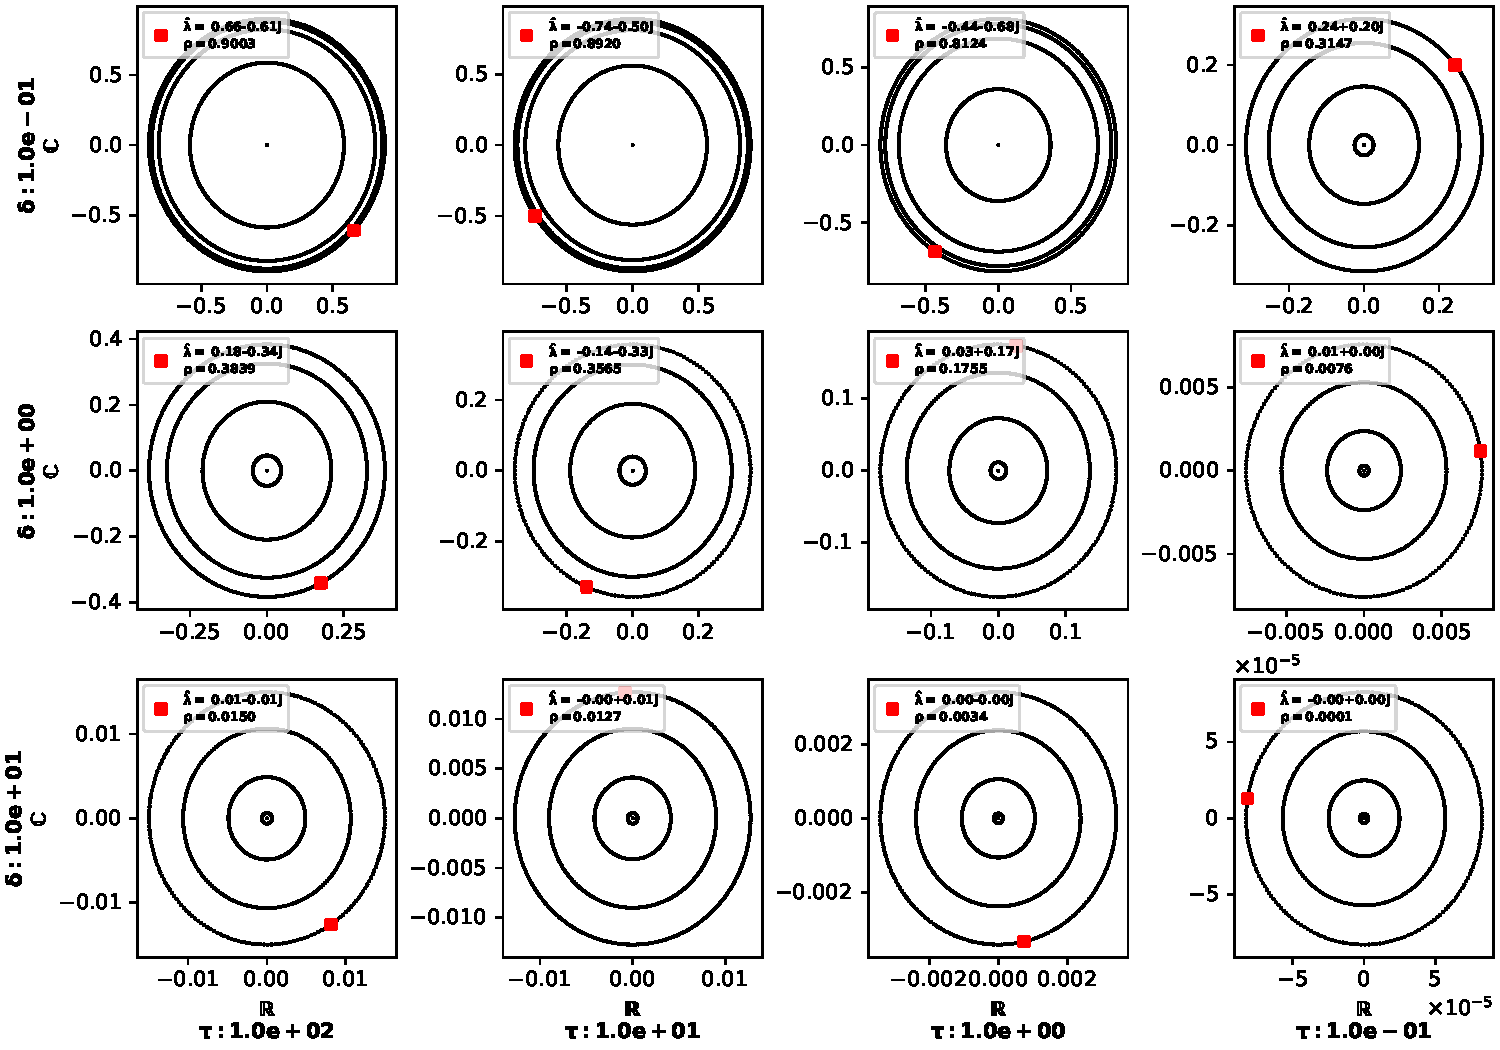
\includegraphics[width=\textwidth]{appendix/eig_plots/oci0.0.pdf}
	\caption{OCI Fourier plots at $c=0$ over various choices of $\delta$ and $\tau$.}
\end{center}
\end{sidewaysfigure}

\begin{sidewaysfigure}
\begin{center}
	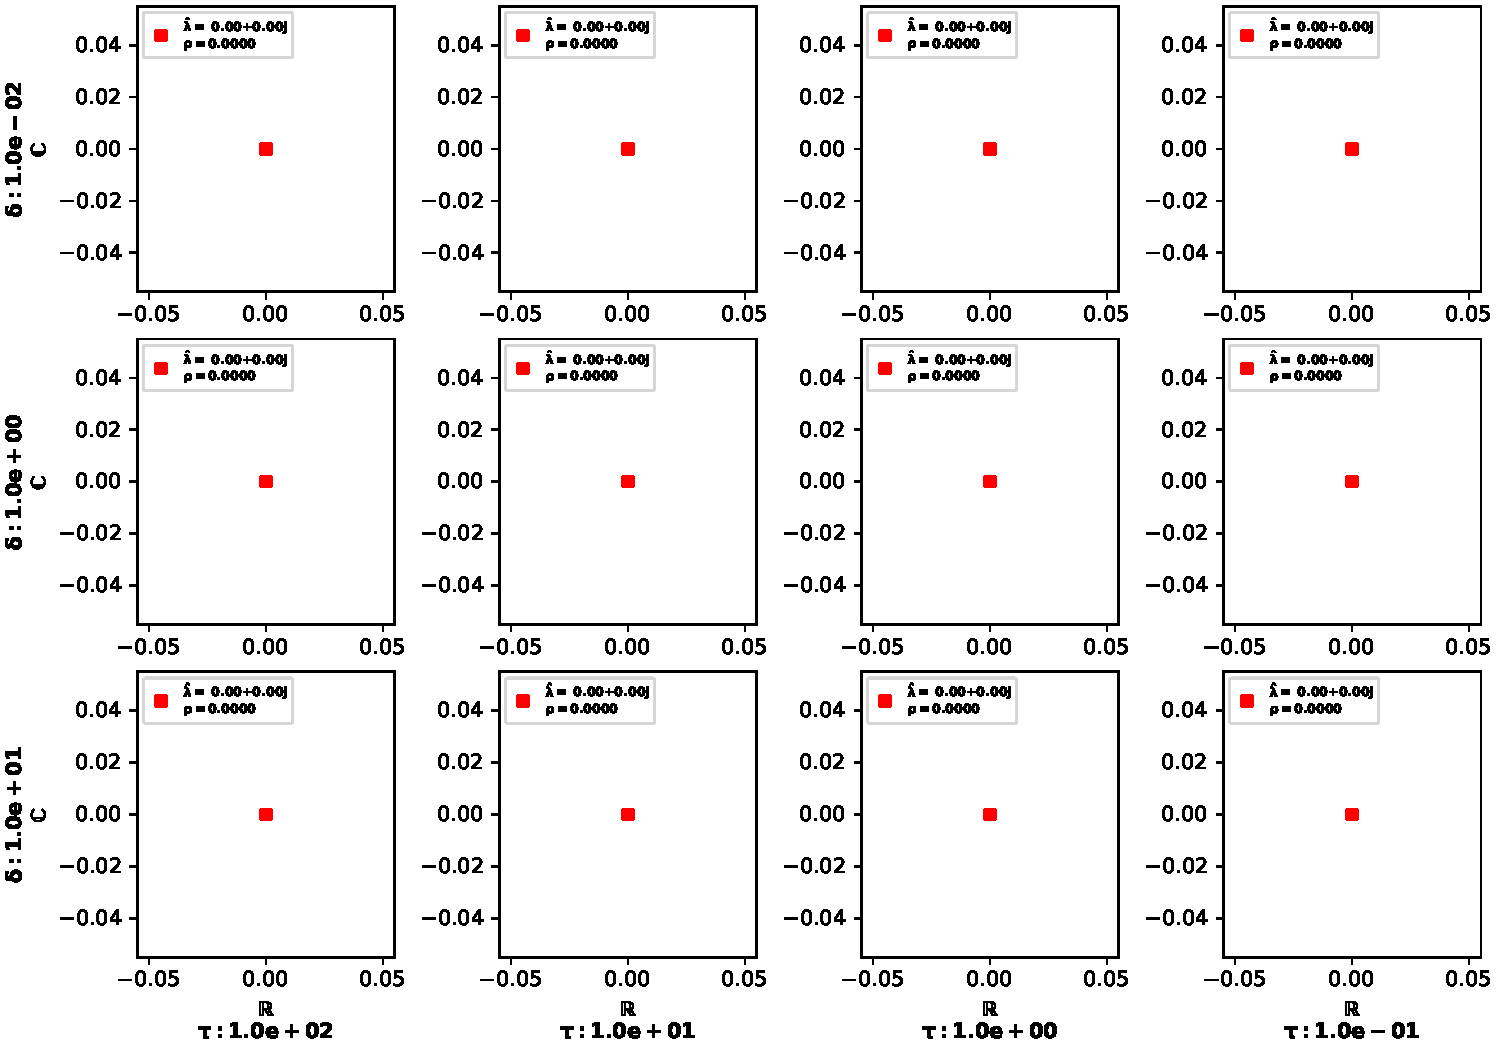
\includegraphics[width=\textwidth]{appendix/eig_plots/si0.0.pdf}
	\caption{SI Fourier plots at $c=0$ over various choices of $\delta$ and $\tau$.}
\end{center}
\end{sidewaysfigure}

\begin{sidewaysfigure}
\begin{center}
	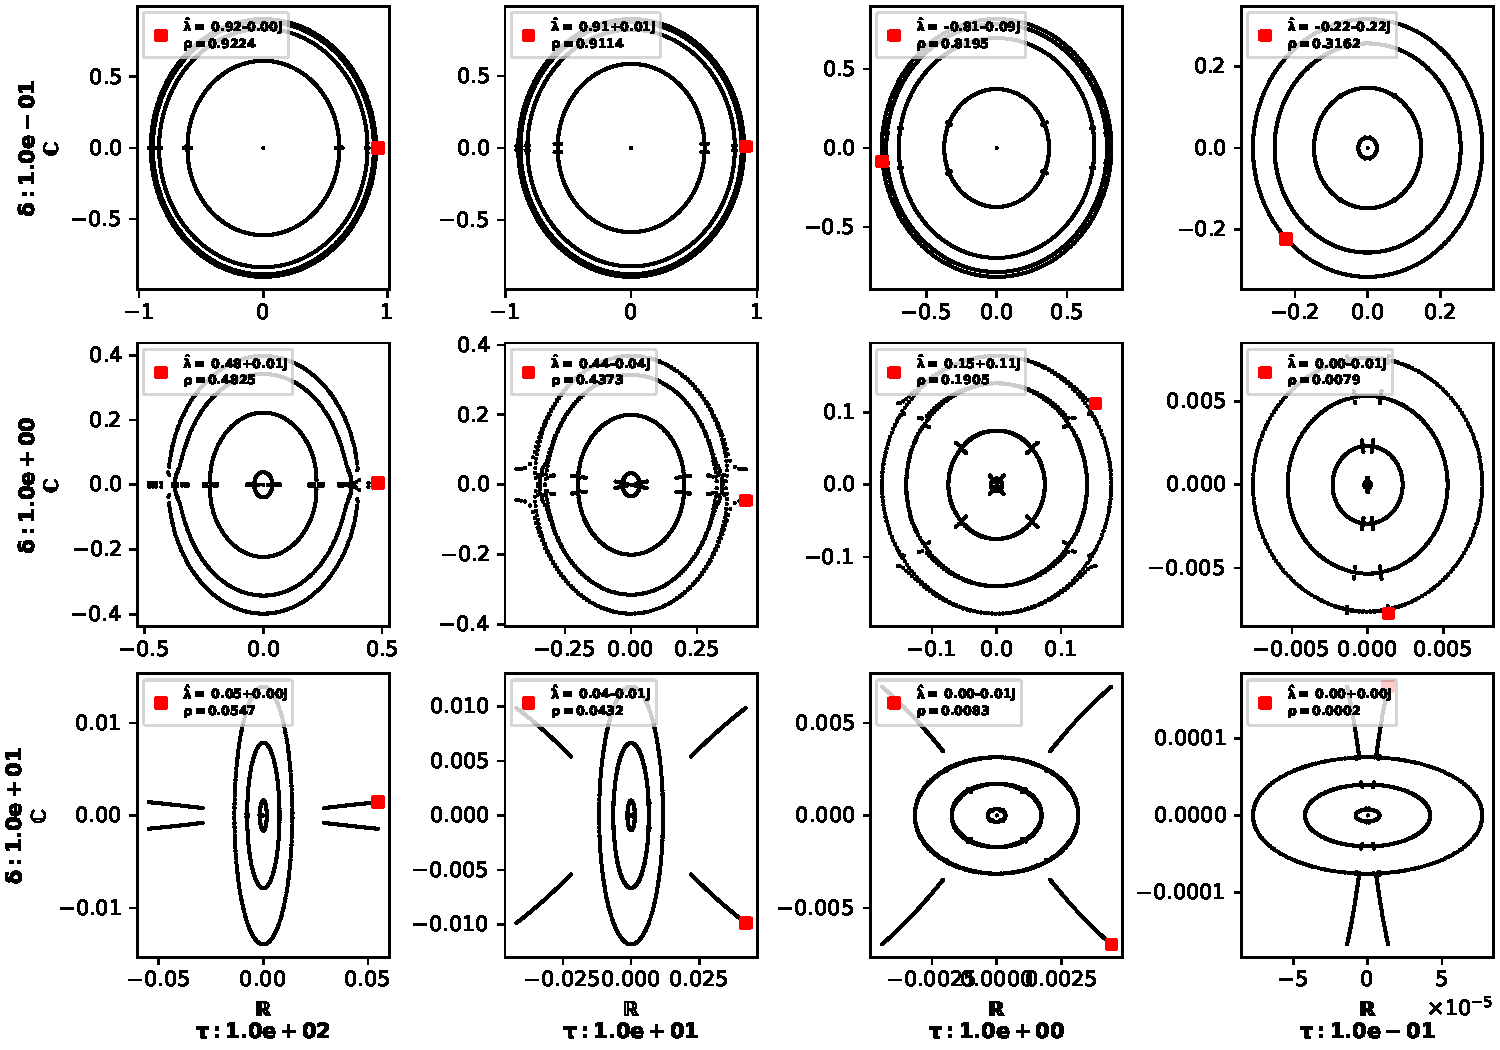
\includegraphics[width=\textwidth]{appendix/eig_plots/oci0.5.pdf}
	\caption{OCI Fourier plots at $c=0.5$ over various choices of $\delta$ and $\tau$.}
\end{center}
\end{sidewaysfigure}

\begin{sidewaysfigure}
\begin{center}
	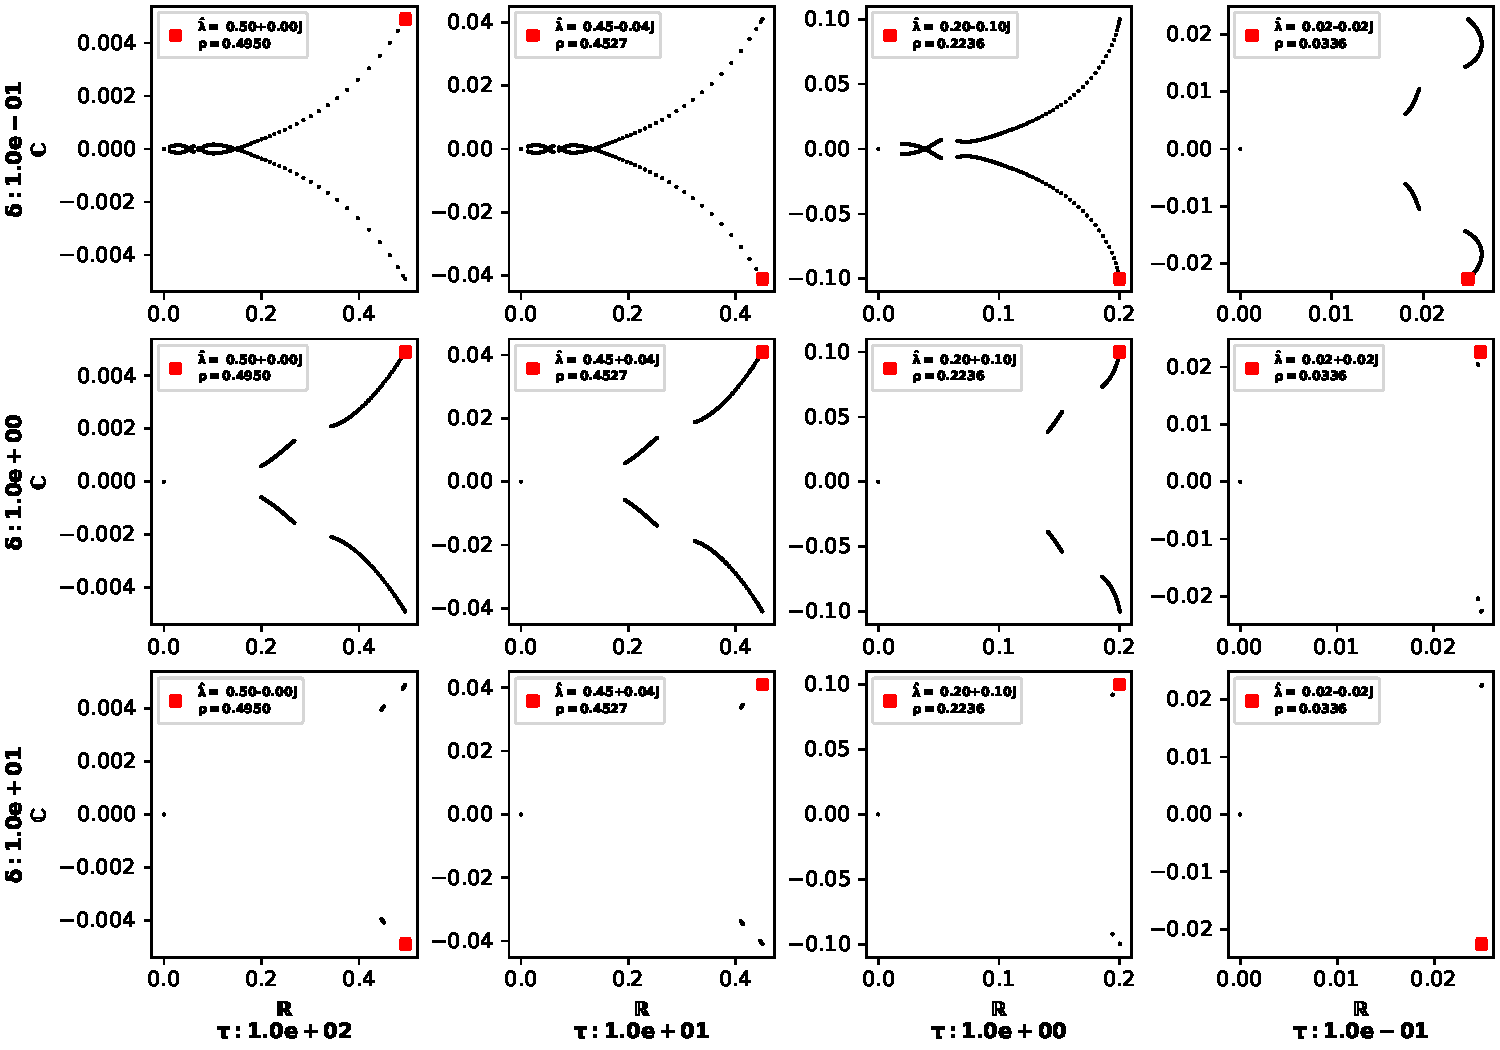
\includegraphics[width=\textwidth]{appendix/eig_plots/si0.5.pdf}
	\caption{SI Fourier plots at $c=0.5$ over various choices of $\delta$ and $\tau$.}
\end{center}
\end{sidewaysfigure}

\begin{sidewaysfigure}
\begin{center}
	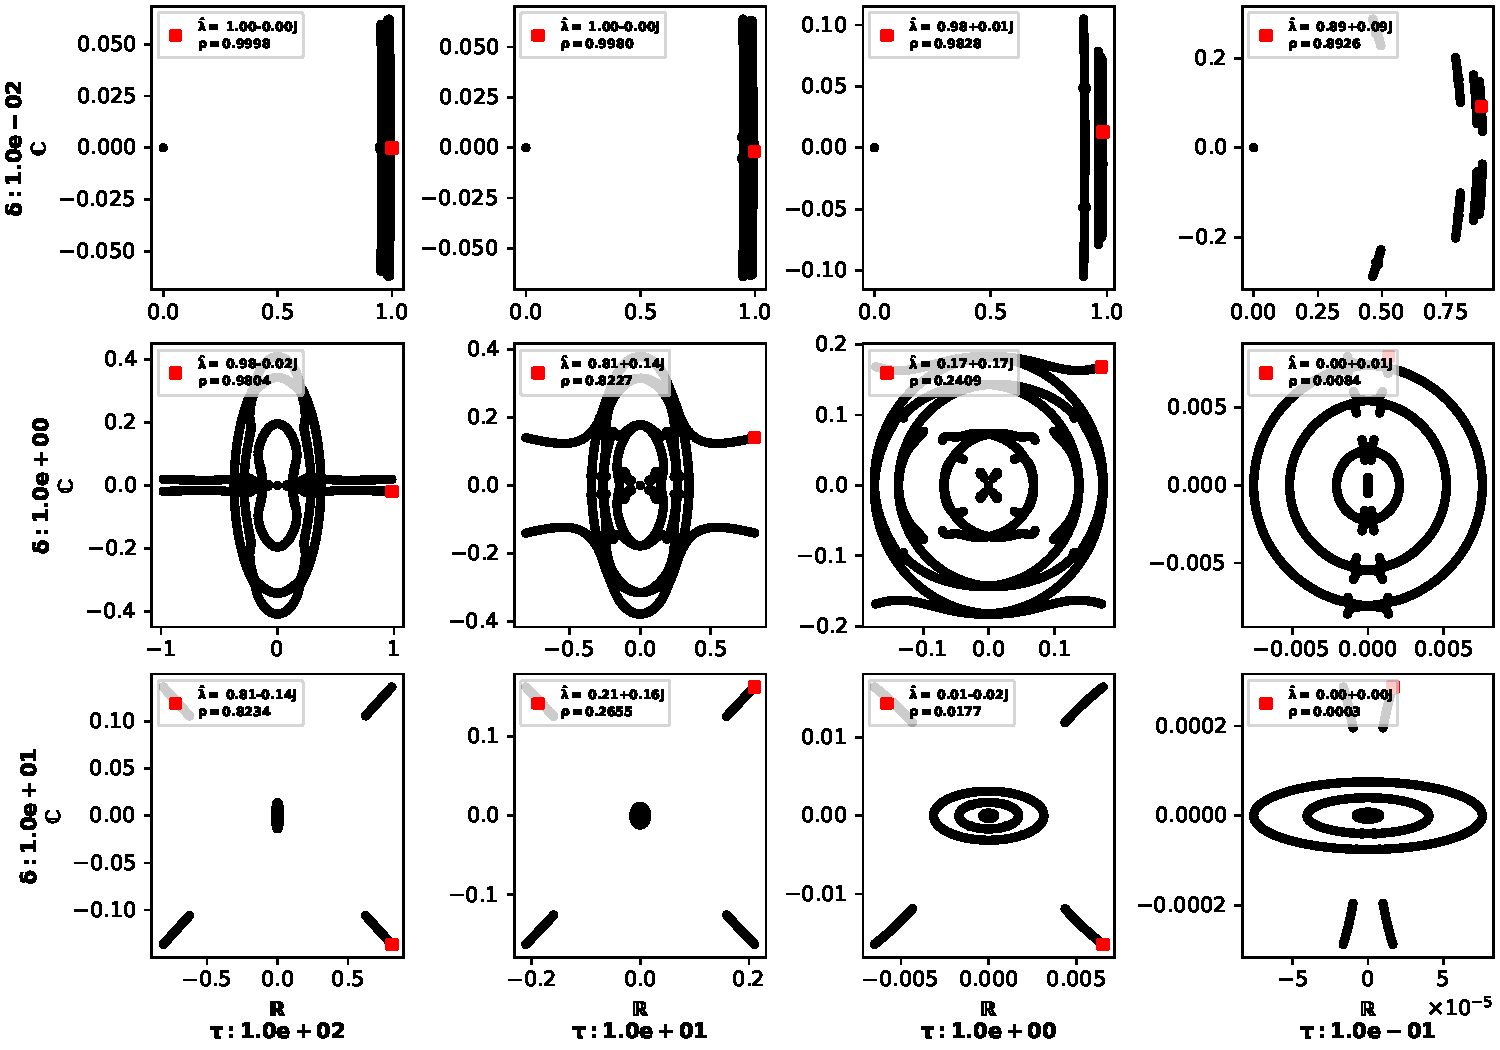
\includegraphics[width=\textwidth]{appendix/eig_plots/oci1.0.pdf}
	\caption{OCI Fourier plots at $c=1.0$ over various choices of $\delta$ and $\tau$.}
\end{center}
\end{sidewaysfigure}

\begin{sidewaysfigure}
\begin{center}
	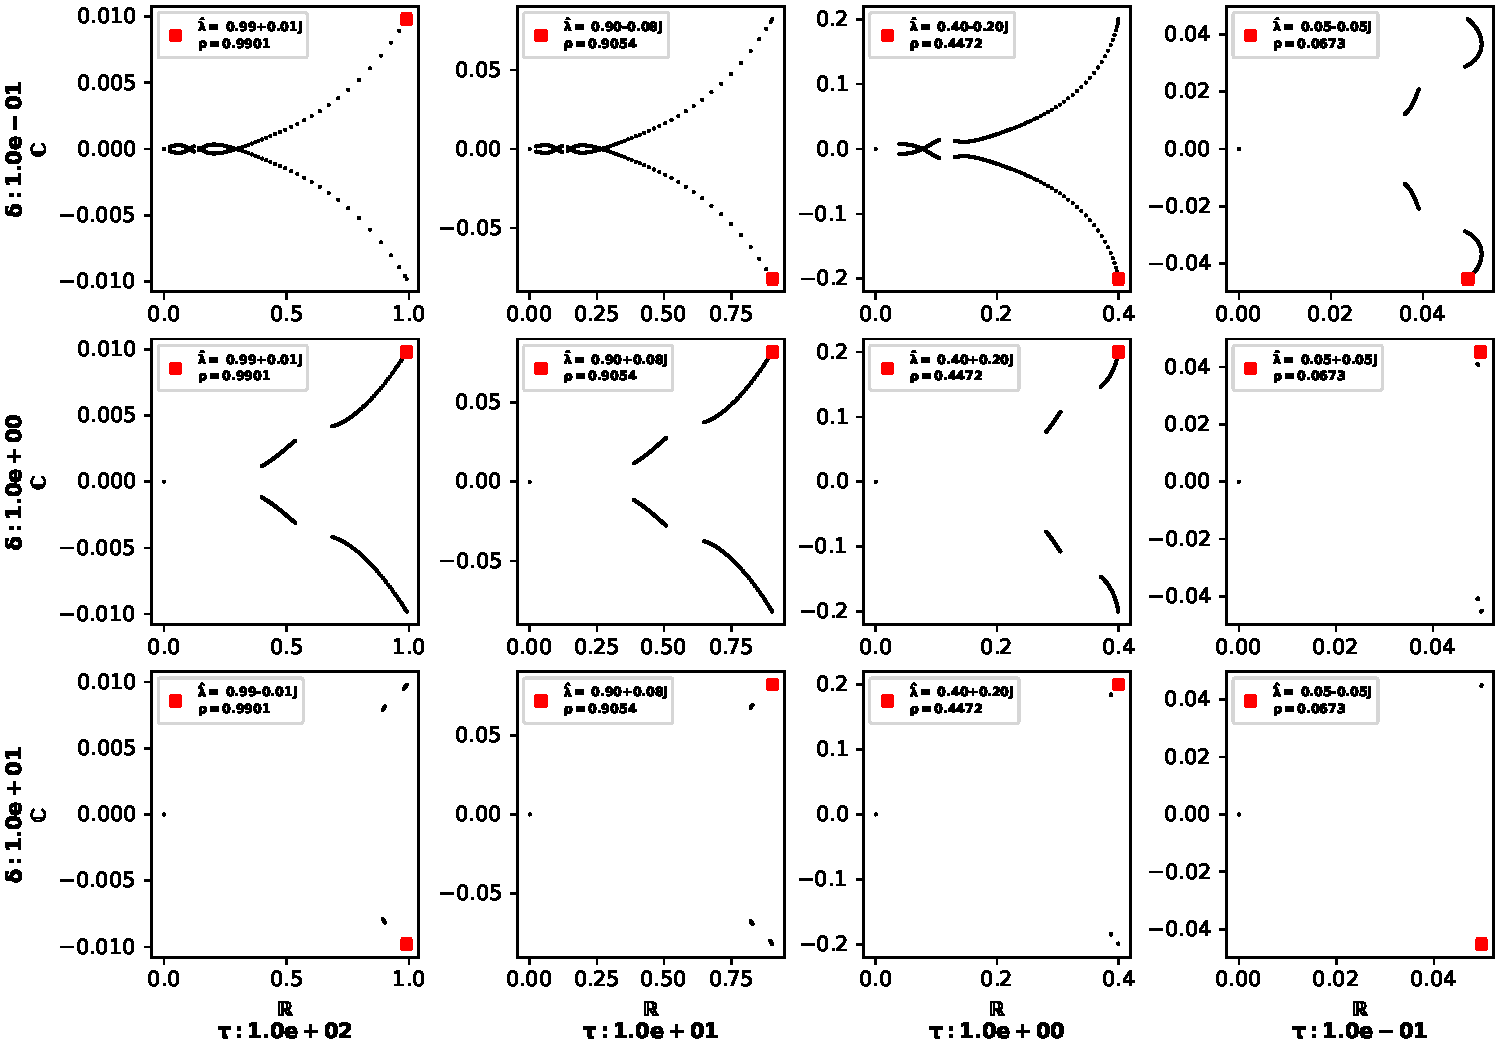
\includegraphics[width=\textwidth]{appendix/eig_plots/si1.0.pdf}
	\caption{SI Fourier plots at $c=1.0$ over various choices of $\delta$ and $\tau$.}
\end{center}
\end{sidewaysfigure}

